\section{Scoping Study with Snowballing Strategy}
\label{rel-work:scoping-snowball}

A systematic mapping used to be a good starting point for further research \cite{kitchenham:2011}, including for Ph.D. studies \cite{kitchenham:2010}. In this mapping, I follow the general framework of a scoping study \cite{arksey:2005}, considering the guidelines for snowballing in systematic literatures proposed by \citeonline{wohlin:2014}. I will describe them better as follows.

The scoping study is a systematic mapping that aims “to map rapidly the key concepts underpinning a research area and the main sources and type of evidence available, [...] especially where an area is complex or has not been reviewed comprehensively before” \cite[p.~21]{arksey:2005}. The methodological framework of a scoping study can be divided into five stages: (i) identifying the research question, (ii) identifying relevant studies, (iii) study selection, (iv) charting data, and (v) collating, summarizing and reporting the results \cite[p.~22]{arksey:2005}.

For identifying relevant studies (second stage), I use the snowballing strategy as the main road to locate additional papers to include for further selection and analysis. This inclusion can be via the reference list or the citations of a paper. The process of identifying new papers from the references’ and the citations’ list are commonly called backward and forward snowballing \cite[p.~1]{wohlin:2014}. Figure \ref{fig:snowballing-schema} presents this procedure schematically. It is important to highlight that several computing education researchers use snowballing strategy in their systematic literature studies as \citeonline{qian:2017}, \citeonline{gomes:2020} and \citeonline{indriasari:2020}.

\begin{figure}[ht!]
\centering

\caption{\textmd{Snowballing procedure schema.}}
\label{fig:snowballing-schema}
\fcolorbox{gray}{white}{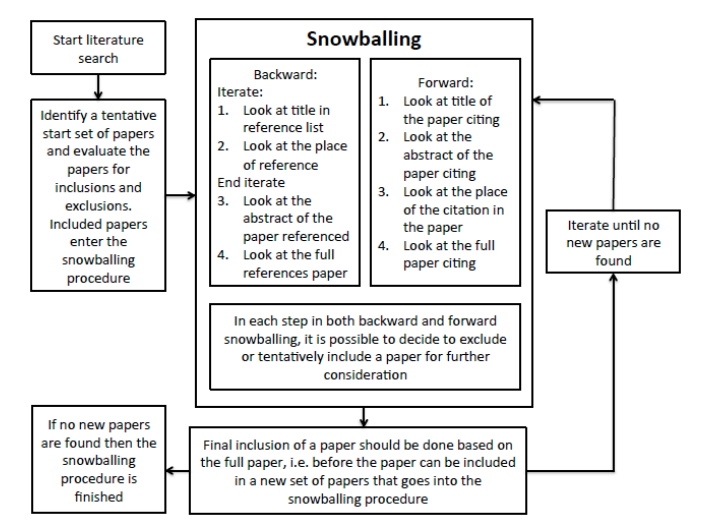
\includegraphics[width=0.9\textwidth]{images/chapter-04/snowballing-schema.png}}

\par\medskip\ABNTEXfontereduzida\selectfont\textbf{Source:} \citeonline{wohlin:2014}.
\end{figure}